
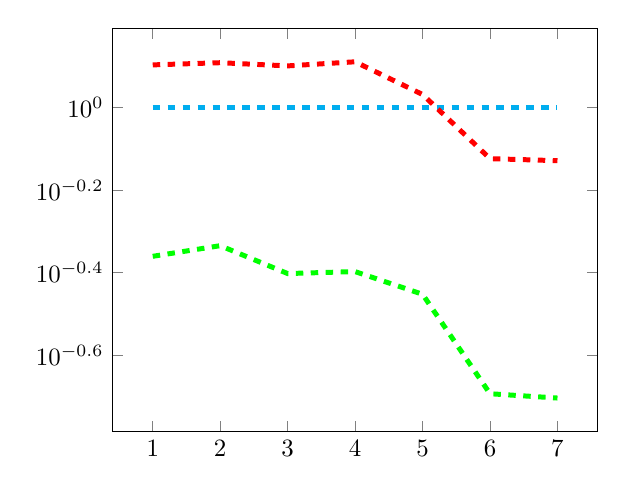
\begin{tikzpicture}[scale=0.9]
\begin{semilogyaxis}
\addplot[dashed,color=cyan,line width=2pt] coordinates {(1,1.0)(2,1.0)(3,1.0)(4,1.0)(5,1.0)(6,1.0)(7,1.0)};
\addplot[dashed,color=red,line width=2pt] coordinates {(1,1.2696589378522027)(2,1.2851766283862935)(3,1.2625808684867894)(4,1.2917380521532753)(5,1.0761562670891636)(6,0.7520969665708053)(7,0.7436166721811954)};
\addplot[dashed,color=green,line width=2pt] coordinates {(1,0.43588971528769166)(2,0.46254089505085505)(3,0.39591454498939355)(4,0.40024010252726017)(5,0.35259169922153205)(6,0.20231611846844239)(7,0.1975322964091681)};

\end{semilogyaxis}
\end{tikzpicture}
